\chapter{TMP}


what made vgg ideal for ssds concept of detection on different scales was the gradual decrease in size of the feature map. We tried to mimic this behaviour by finding a suitably sized feature maps in other networks, which can complicate the implementation, especially in block architectures.


\section{Reimplement SSD on other base}
\subsection{ResNet-SSD}
\begin{figure}
    \resnetSSD
    \caption{SSD detector build on ResNet base. Depth of classification convolutions depends on number of classes (C). For detailed description of \textit{Layers} see \cref{fig:resnet_arch}.}
    \label{fig:resnetSSD}
\end{figure}

\subsection{Xception-SSD}


\begin{figure}
    \xceptionSSD
    \caption{SSD detector build on Xception base. Depth of classification convolutions depends on number of classes (C). Note that ReLU activation and batch normalization functions are omitted from this chart. For detailed description of blocks see \cref{fig:xception}}
    \label{fig:xceptionSSD}
\end{figure}


\subsection{Xception-B-SSD and Xception-C-SSD }
\begin{figure}
    \xceptionBSSD
    \caption{SSD detectors build on our modified Xception bases. We reduced the output depth of blocks 3 to 7 from 728 to 256 and as a consequence doubled the size of feature map. In version C, we also omitted blocks 5,6,7 and moved feature extraction from block 11 to block 10. For details on extra layers, classification and location layers see \cref{fig:xceptionSSD}}
    \label{fig:xceptionBSSD}
\end{figure}


\subsection{NasNet-SSD}

\begin{figure}
    \nasnetSSD
    \caption{SSD detector build on NASNet base. Depth of classification convolutions depends on number of classes (C). For detailed description of cells see \cref{sec:nasnet}}
    \label{fig:nasnetSSD}
\end{figure}


\subsection{Train results}
\begin{table}
    \begin{tabular}{c|c|c}
                            & coco      & small \\
        Resnet34-SSD        & 32.4      & 47.3  \\
        Resnet50-SSD        & 32.7      & 48.7  \\
        Resnet101-SSD       & 32.8      & 45.7  \\
        Xception-A-SSD      & 26.8      & 37.8  \\
        Xception-B-SSD      & -         & 48.4  \\
        Xception-C-SSD      & -         & x     \\
        NASNet-mobile-SSD   & -         & 36.9  \\
    \end{tabular}
    \caption{mean average precision, conf thr 0.2, IoU 0.5,  (400 epochs), 300x300 scaled random crops}
    \label{tab:map}
\end{table}

\begin{figure}
    \centering
    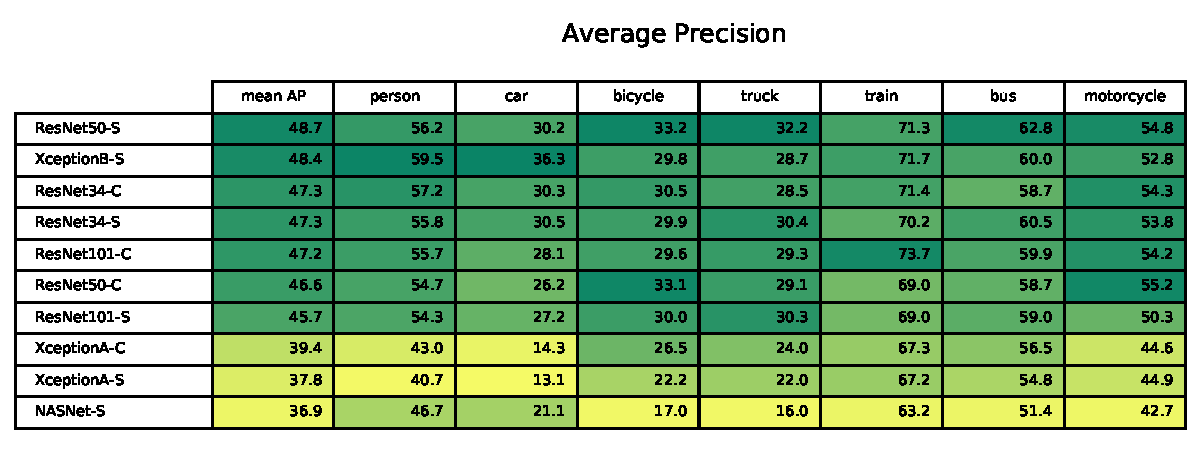
\includegraphics[width=\textwidth]{img/ap}
    \caption{AP, small 7 class dataset S, coco dataset C}
    \label{fig:ap}
\end{figure}


\begin{table}
    \begin{tabular}{c|c|c}
                    & 81cls     & 8cls  \\
    Resnet34        & 31.1M     & 24.4M \\
    Resnet50        & 45.5M     & 28.7M \\
    Resnet101       & 64.5M     & 47.7M \\
    Xception-A      & 40.6M     & 25.7M \\
    Xception-B      & x         & 19.2M \\
    Xception-C      & x         & 18.5M \\
    NASNet          & 17.3M     & 7.6M  \\
    VGG             & 34.3M     & x \\
    \end{tabular}
    \caption{total number of parameters}
    \label{tab:parameters}
\end{table}

fps
testing done on GTX 1080 Ti
10000 images, 300x300 
224x224 for nasnet
times include NMS
batch 16


\section{something, use video continuity???}





\chapter*{Experiments}
\todo{something
}
\section{Experiments with Single-Shot Detector}
\label{chapt:experiments}
Based on our needs in terms of speed and accuracy we decided to base our first set of experiments on SSD detector (\cref{sec:ssd}). The decision between SSD and YOLO (\cref{sec:yolo}) was made by personal experience with SSD detector and it's application in real-time video analyses. However we decided replace the originally used VGG-16 network (\cref{sec:VGG}) and instead build our detector atop the faster ResNet classifier (\cref{sec:resnet}). We started our experiments with small ResNet-18, but the block structure of ResNet allows for using the same implementation of SSD-ResNet on any standard ResNet size, by using outputs of individual blocks as detectors inputs.

This section will describe the process of creating our SSD-ResNet network and multiple experiments performed in the course of development. We experimented with different methods of training the network, speed of inference based on the multiple parameters, we also tried training on artificial data for real-life applications.


\subsection{Building SSD based on ResNet}
The task of building full SSD detector can be a little overwhelming without prior experience of building similar networks, so we decided to start with ResNet classifier and add localization layer. After successful implementation we went on to implement full detector. 

In order to verify the functionality and precision of our implementation we started by designing and implementing a simple artificial data generator. We chose to avoid using any common datasets because of non-trivial pre-processing requirements. The detector will be trained on real data after it's functionality and viability are proven.

\subsubsection{Testing data}
We will test our implementation on artificial data generated on demand. We implemented simple generator for geometric shapes. We used squares, triangles and circles with fully randomized position, size, color and thickness. The triangles are in general position only conditioned by minimal ratio of circumference to area.
To make dataset more complex, shapes are drawn over random background composed of the segments of the same shapes. The background shapes are never fully in the picture background. The example image seen be seen in \todo{example data}.



% feature map sized
% block1: 56x56
% block2: 28x28
% block3: 14x14
% block4: 7x7

% unlike original SSD on VGG-16 we decided to start with this basic setup without adding more feature layers, because we are interested in small objects on surveillance video and not for recognizing large objects on photographs.

% \begin{figure}
%     \centering
%     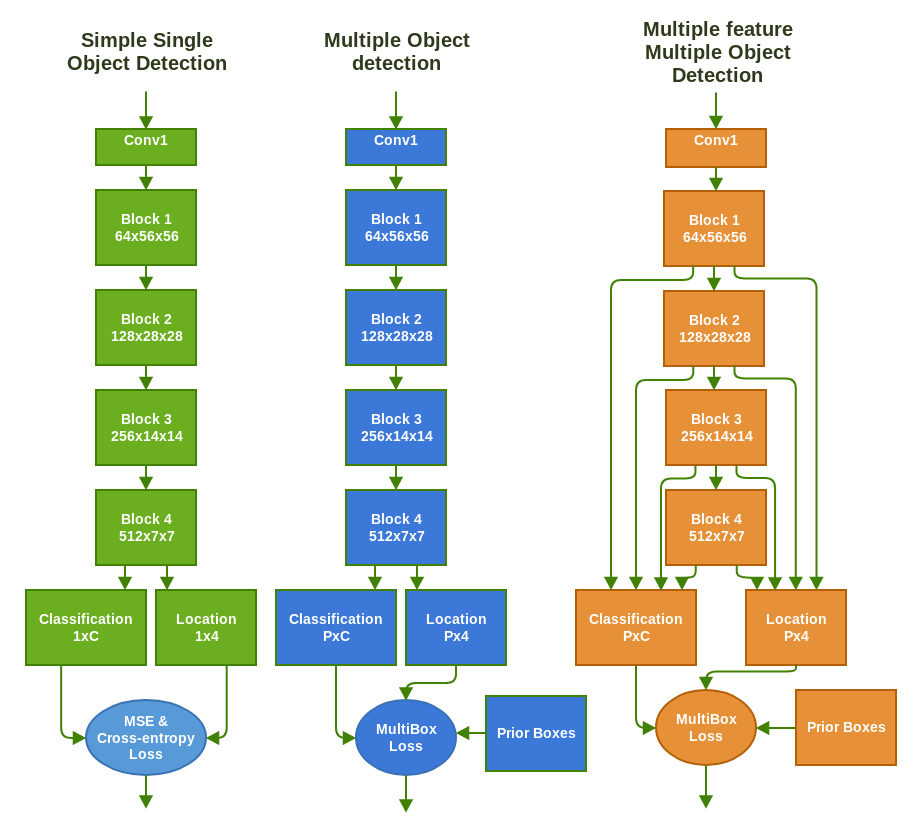
\includegraphics[width=\textwidth]{img/resnets.png}
%     \caption{High level structure of resnet with SSD}
%     \label{fig:resnet}
% \end{figure}

\subsubsection{Simple detector for one object}
The first step towards detector network is classification network. Ussually the detectors initialized with weights from classification networks pretrained on imagenet or similar dataset and then the multibox head is trained. Many pretrained classifiers are publicly available and included in popular frameworks like PyTorch or TensorFlow.

We decided  to go one step further and start with network that combines classification and detection for one object. We started by taking PyTorch implementation of ResNet and modified last layers of the network accordingly. 


optimizer = Adam(lr=0.001, betas=(0.9, 0.999), eps=1e-08, weight decay=0)
class loss = CrossEntropyLoss
loc loss = MSELoss output of NN with absolute coordinates of ground truth box normalized to -1,1 

resnet 18: in addition to fully connected layer we use feature map before avg pooling as input to 7x7 convolution with 4 filters (4 coordinates) Only output of B4 on picture \cref{fig:resnet_arch} 

test on 10000 images
results: class accuracy: over 99.73\%
class loss: 0.0132
location loss (mean squared error): 0.0043


% \begin{figure}
%     \centering
%     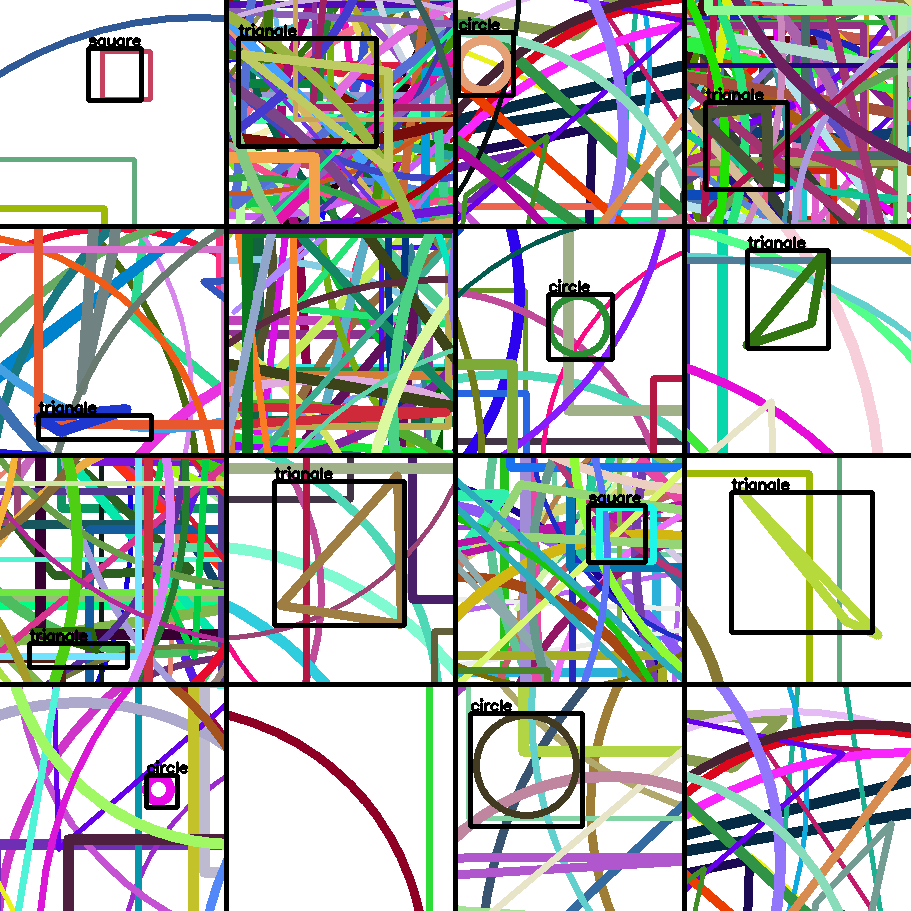
\includegraphics[width=\textwidth]{img/simple_detection.png}
%     \caption{Detections by simple model 1 7x7 feature map to 4 coordinates and fully connected for class}
%     \label{fig:my_label}
% \end{figure}

\subsubsection{Full SSD, convolution and multiple feature layers}
Training SSD clear vs pretrained
batch size 256, batches per epoch 500
% \begin{table}[]
% \begin{tabular}{llll}
%  Epochs &  random mAP & pretrained mAP & imgNet pret. mAP \\
%  1 & 0.11 & 0.76 & 0.53 \\
%  &  & &\\
%  &  & &
% \end{tabular}
% \caption{bla bla}
%     \label{tab:Comparison of training}
% \end{table}




\subsection{Applying SSD trained on artificial dataset to realistic images}
SSD 6cls random $>96$
same SSD on imgs on coco - 93

SSD 4cls random $>97$
same SSD on imgs on coco 87


SSD coco mAP 25.78

SSD coco subset [1 person
2 bicycle
3 car
4 motocycle
6 bus
7 train
8 truck] mAP

\subsection{Measuring the impact of number of classes}

\section{Speeding up video procesing}